\documentclass[11pt]{amsart}
\usepackage[T1]{fontenc}
\usepackage[english]{babel}
\usepackage{graphicx}
\usepackage{fancyvrb}
\usepackage{geometry}[margin=0.5in] % page geometry
\usepackage{xcolor} % colors
\usepackage{tikz} % drawing
\usepackage{hyperref} % hyperlinks
\usepackage{enumerate}
\renewcommand{\arraystretch}{2}
\title{Project Writeup}

\author{S. Chettih}

\begin{document}
\maketitle
\section{Setup, training, and deployment on SageMaker}
\subsection{Notebook Instance}
I chose a \textbf{ml.t3.medium} instance for my Jupyter notebook (Fig \ref{fig:init}). I chose this instance type because it is eligible for the AWS free tier, and thus inexpensive, while still powerful enough for the code I planned to run on it. I knew I'd be installing packages, and downloading, unzipping, and uploading images using this instance, but model tuning, training, and deployment would happen on other instances. I also wanted the fast launch capability of ml.t3.medium, since I anticipated stopping and starting the notebook multiple times in the course of the project.
\begin{figure}[h]
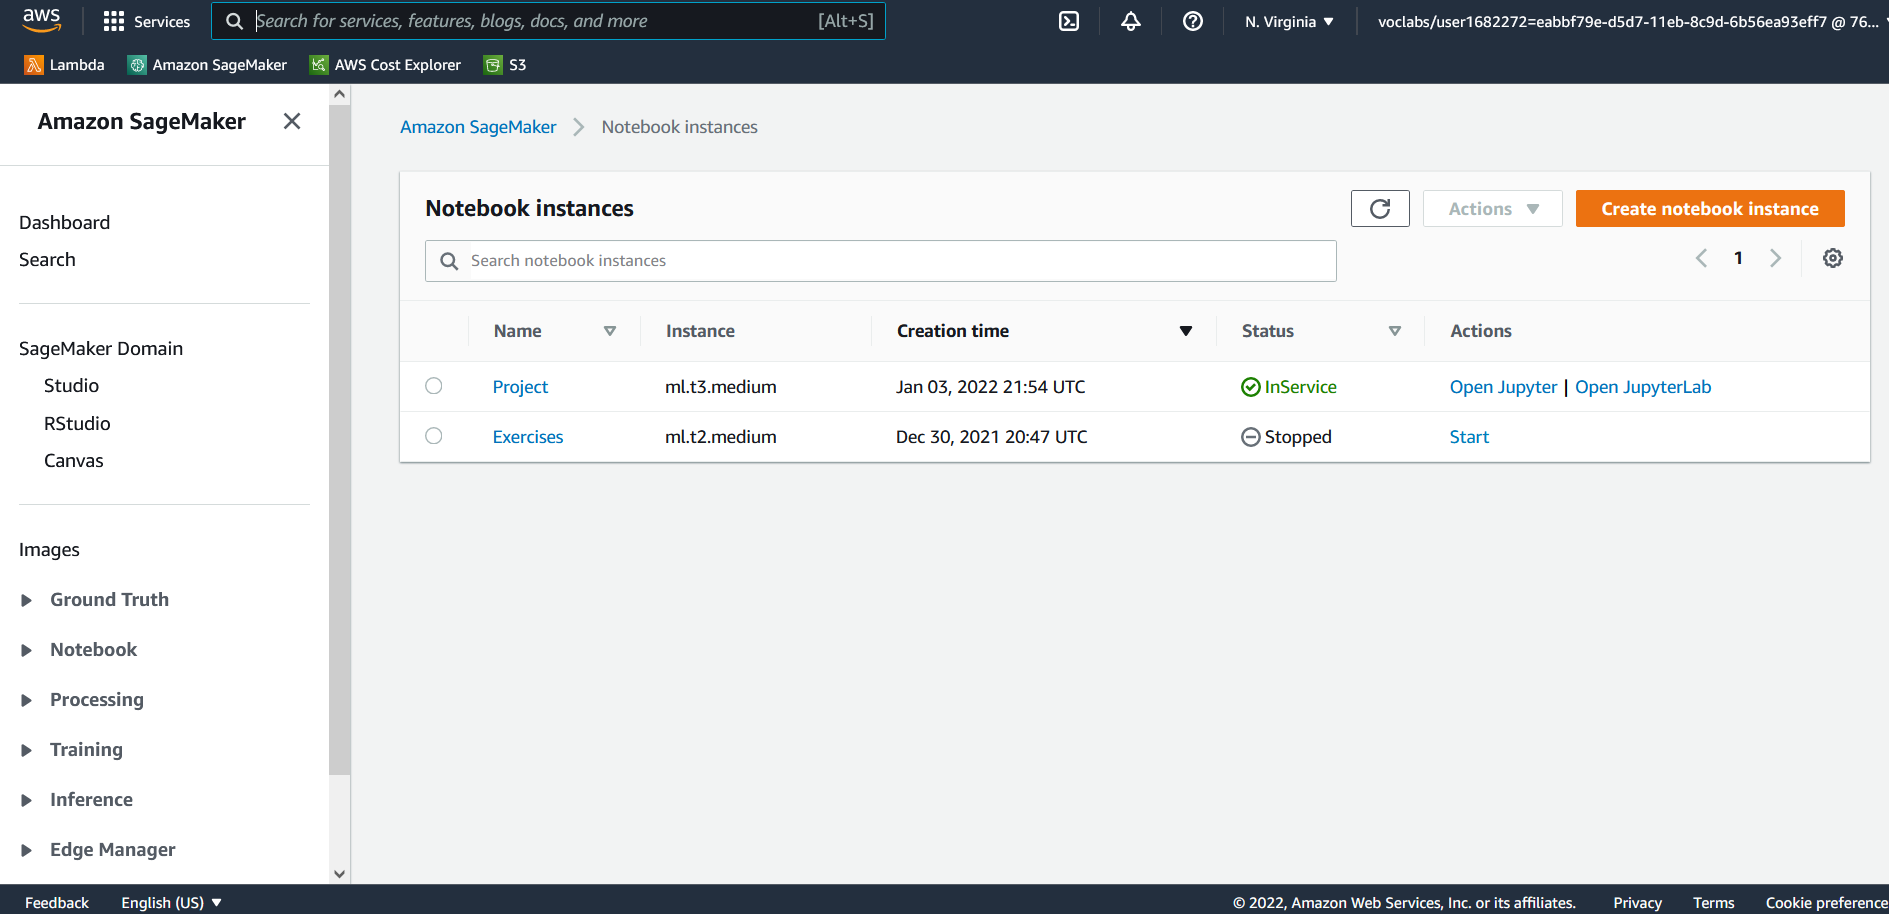
\includegraphics[width=\textwidth]{initial_setup.png}
\caption{Notebook instance}
\label{fig:init}
\end{figure}
\subsection{S3 Bucket}
I created the S3 bucket \texttt{operationalizing-ml-project} to copy the data into (Fig \ref{fig:bucket}). I changed the references in \verb^train_and_deploy-solution.ipynb^ to point to this bucket, and I uploaded the unzipped dogImages dataset to \newline
 \verb^s3://operationalizing-ml-project/dogImages/^.
\begin{figure}[h]
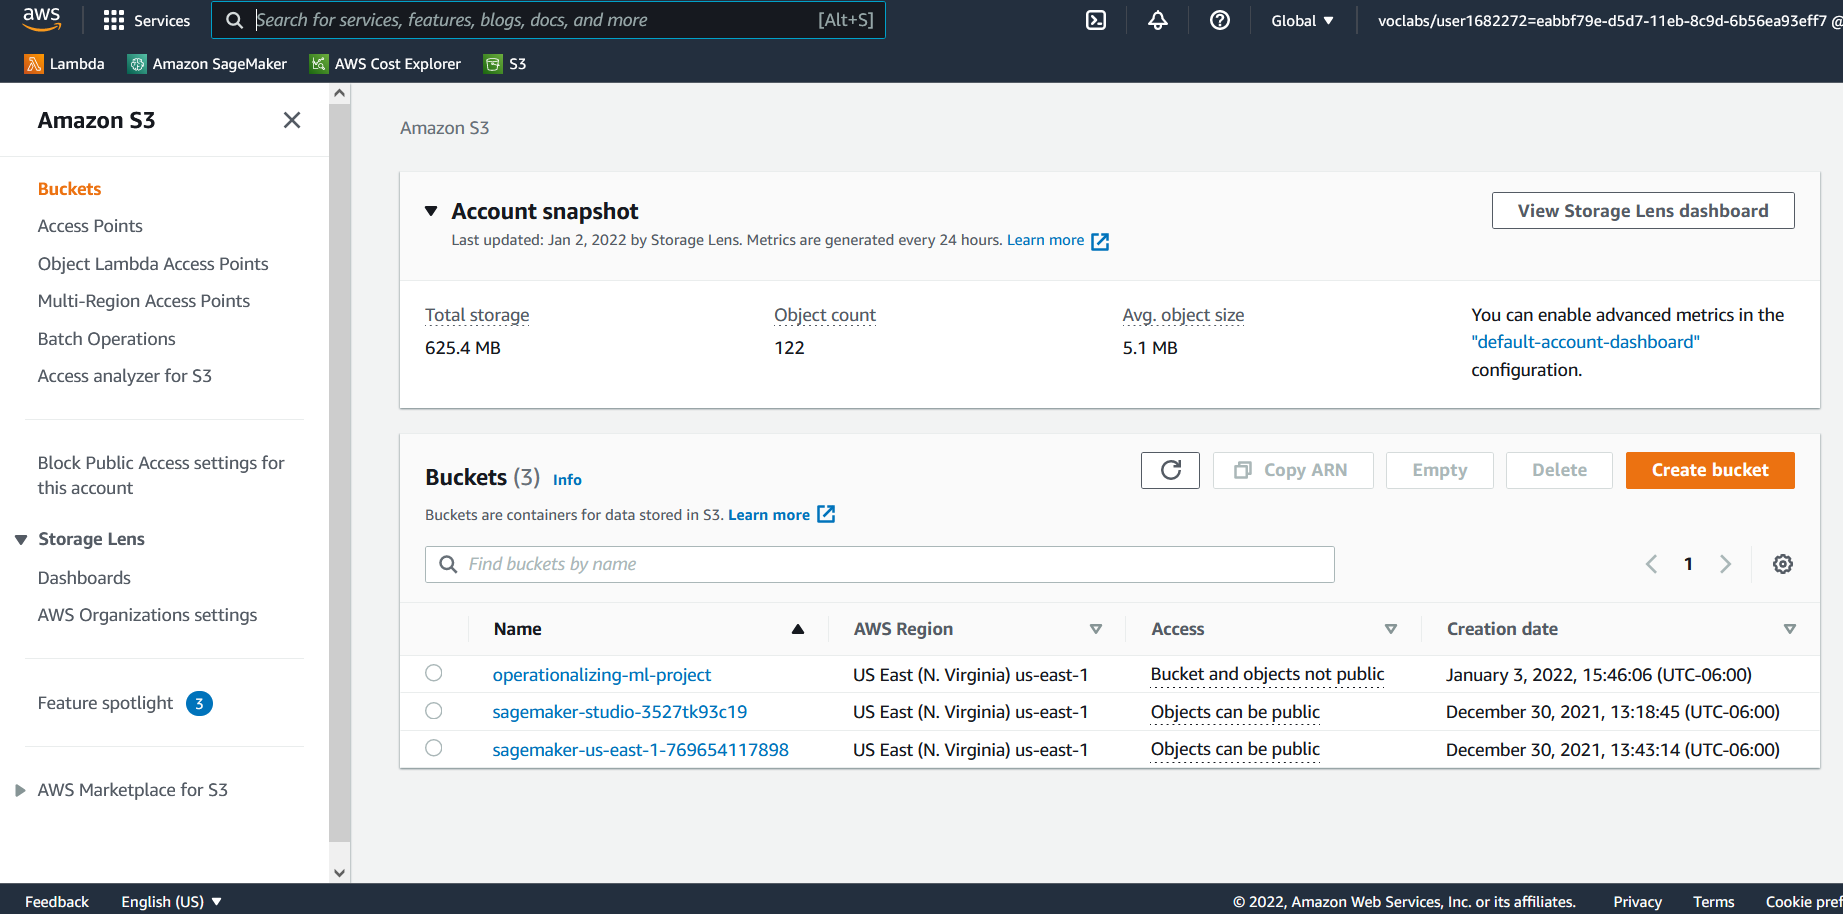
\includegraphics[width=\textwidth]{s3_bucket.png}
\caption{S3 Bucket}
\label{fig:bucket}
\end{figure}
\subsection{Training and Deployment}
For hyperparameter tuning I used an \textbf{ml.m5.xlarge} instance with 2 jobs. This instance is part of the free tier for training in SageMaker, and from experience I knew this would take about 25-30 min, which was acceptable. The best hyperparameters were a batch size of 32 and a learning rate of approximately 0.0373.

I used an \textbf{ml.m5xlarge} instance to train the estimator, using the best hyperparameters from my tuning job. Once it was trained, I deployed the model to an endpoint on a \textbf{ml.m5.large} instance. I chose this type of instance because it wouldn't need to handle very many or very large inference queries. The endpoint's name was \newline\texttt{pytorch-inference-2022-01-03-23-03-42-737} (Fig \ref{fig:single}).
\begin{figure}[t]
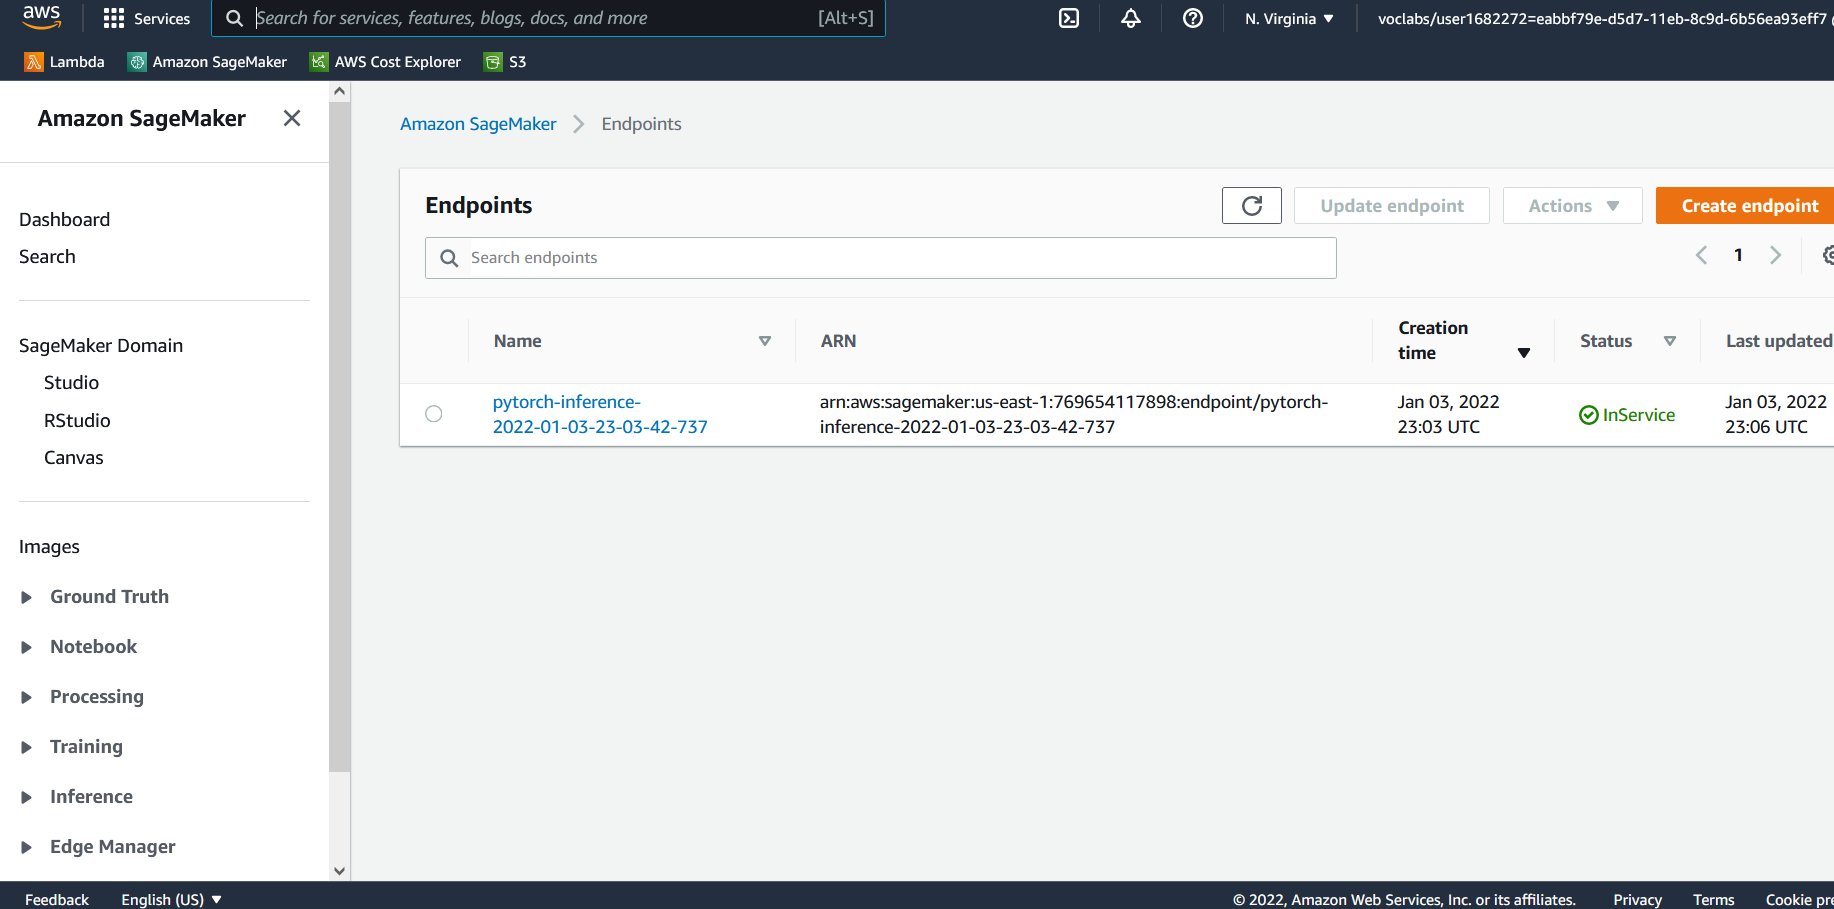
\includegraphics[width=\textwidth]{single_endpoint.png}
\caption{Endpoint from Single-Instance Training}
\label{fig:single}
\end{figure}

After running the rest of the notebook, to confirm that the endpoint could perform inference, I went back and used 4 instances of type \textbf{ml.m5.xlarge} to perform multi-instance training. Once it was trained, I deployed to an endpoint on a \textbf{ml.m5.large} instance. The endpoint's name was \texttt{pytorch-inference-2022-01-04-03-32-53-734} (Fig \ref{fig:multi}).
\begin{figure}[h]
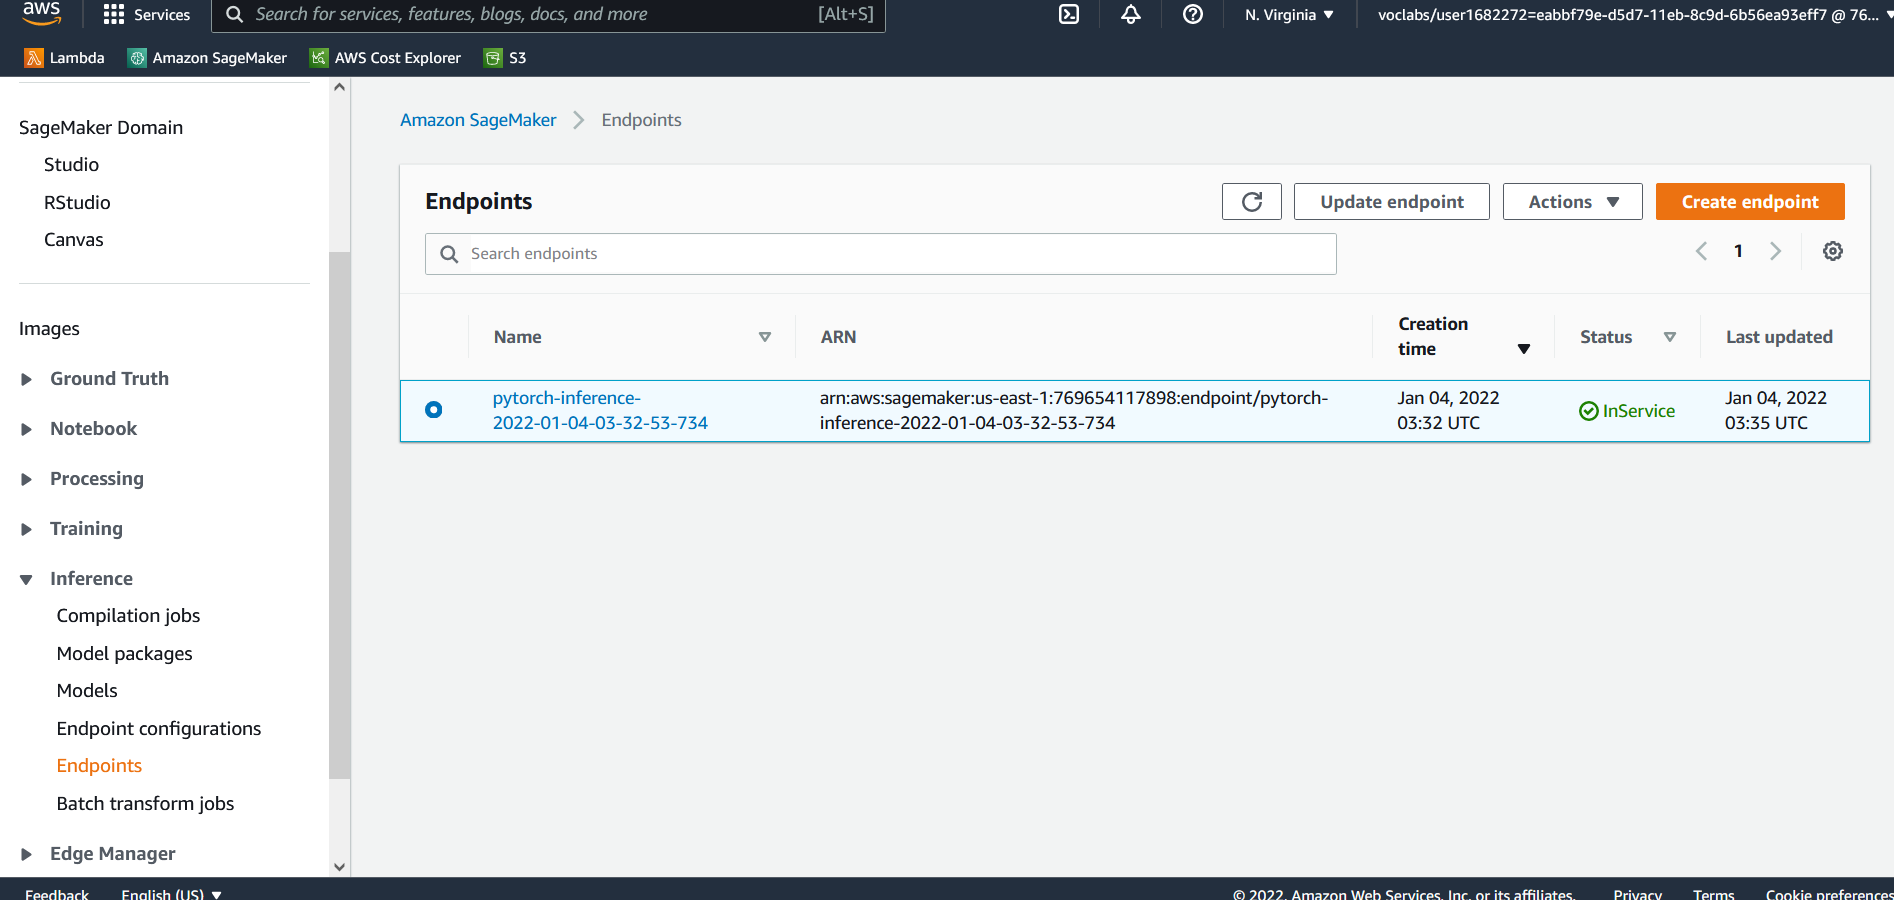
\includegraphics[width=\textwidth]{multi_endpoint.png}
\caption{Endpoint from Multi-Instance Training}
\label{fig:multi}
\end{figure}
\begin{figure}[h]
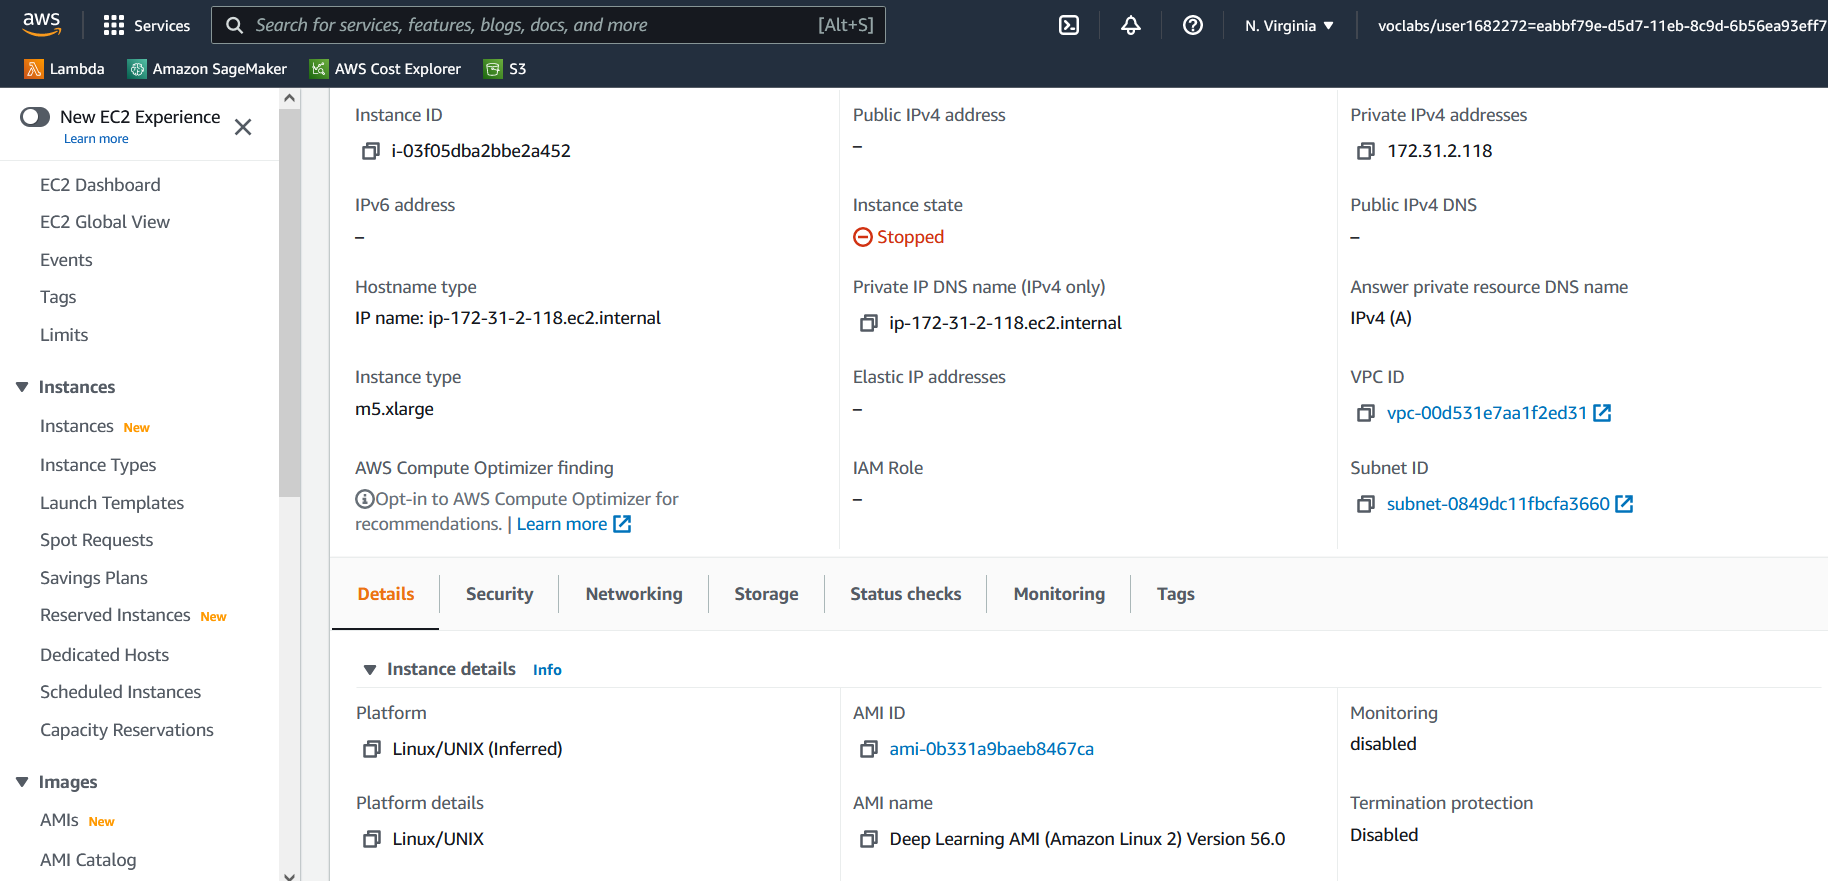
\includegraphics[width=\textwidth]{ec2_instance.png}
\caption{EC2 Instance}
\label{fig:ec2}
\end{figure}

\section{EC2 Training}
\subsection{EC2 Setup}
I chose the Deep Learning AMI (Amazon Linux 2) Version 56.0, running on an \textbf{m5.xlarge} instance (Fig \ref{fig:ec2}). I knew this would be powerful enough to complete model training in a reasonable amount of time, and it wouldn't bankrupt my account if I needed to leave it on for a few hours to troubleshoot.

I launched the instance, downloaded the dataset, and trained the model, saving it in the TrainedModels directory (Fig \ref{fig:dir}).
\begin{figure}[h]
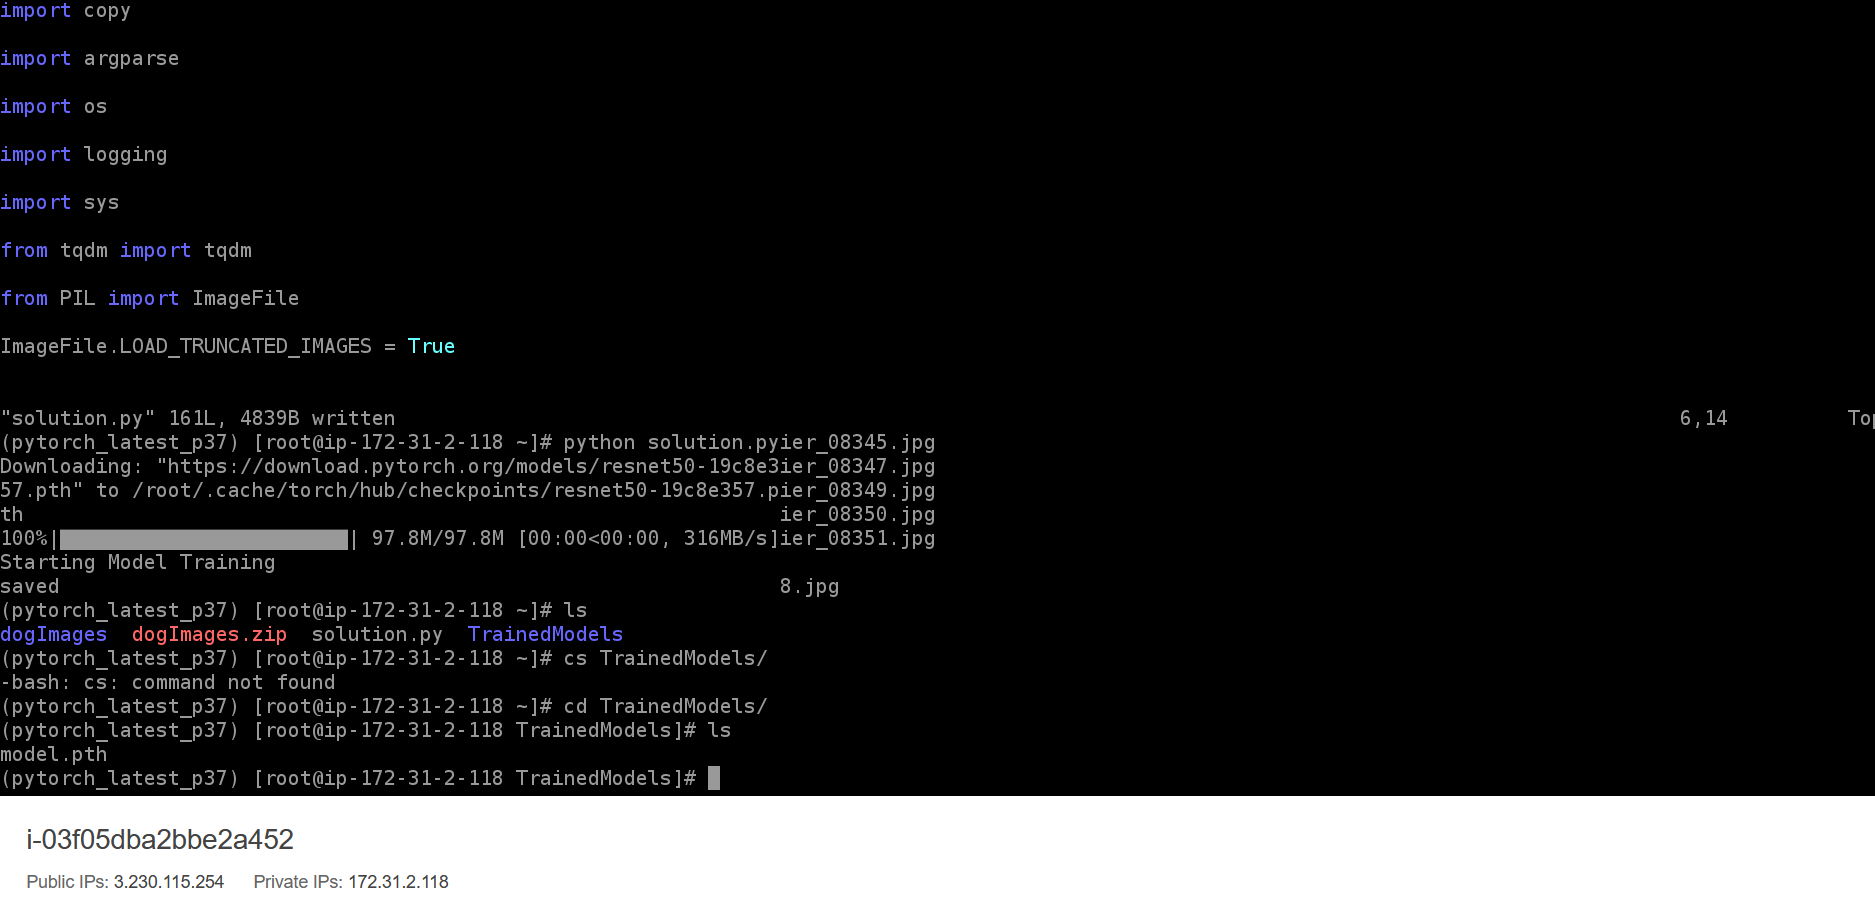
\includegraphics[width=\textwidth]{ec2_model_path}
\caption{TrainedModels Directory}
\label{fig:dir}
\end{figure}


\subsection{EC2 vs SageMaker}
The code in \verb^ec2train1.py^ is similar to \verb^train_and_deploy-solution.ipynb^ plus \verb^hpo.py^, with a few key differences. Firstly, the EC2 script performs all training locally. Contrast this to SageMaker, where the training data, model, and output are stored on S3, and estimators are fit on separate instances from the notebook where the code is run. This is part of why the EC2 script doesn't need a parser or a main function. In SageMaker, the parser passes on the learning rate and batch size, as well as the training, model, and output directories to the main function. In EC2, all of these are simply specified in the script. This is only possible because the dataset is available locally, the training is done locally, and the model can be saved locally. Finally, it's not possible to directly deploy the trained model to an endpoint from EC2. We only know how to deploy endpoints from models within SageMaker, so we'd need to get the model from the EC2 instance into SageMaker first before we could deploy an endpoint to perform real-time inference.

\section{Lambda Function Setup}
I used the \verb^lambdafunction.py^ starter file to set up a Lambda function called \texttt{dog-breed-prediction}. The function first creates a Boto3 client. This allows the function to interact with other AWS applications, like SageMaker. The function uses the client to invoke the endpoint I deployed from the multi-instance trained model, called \texttt{pytorch-inference-2022-01-04-03-32-53-734}. It expects the input/image in JSON format, and it returns a JSON file. This JSON file has a status code of 200 and the prediction from the endpoint in the key `body'.

\section{Lambda Function Security and Testing}
\subsection{Testing}
After attaching the appropriate permissions to the Lambda function role, I ran a successful test of my lambda function (Fig \ref{fig:test}). The returned list is 
{\small
\begin{align*}
[&-8.925518989562988, -4.890507698059082, -3.2437384128570557, -1.4612047672271729, \\
&-1.6248699426651, -6.121954441070557, -2.5580923557281494, -2.1696574687957764,\\&
 -7.28581428527832, 0.02648542821407318,  0.19917014241218567, -5.017480373382568,\\&
  -3.6260993480682373, 1.1632394790649414, -5.876077175140381, -2.9551069736480713, \\&
  -5.999130725860596, -2.639396905899048, -4.315248966217041, -0.2771189212799072, \\&
  -4.760954856872559, -1.261879563331604, -8.60474681854248, -6.055394649505615, \\&
  -5.513672828674316, -8.68757152557373, -4.001145839691162, -4.517764568328857, \\&
  -5.7072601318359375, -2.0146870613098145, -5.00324010848999, -4.045901298522949, \\&
  -7.567681789398193, -1.9930708408355713, -8.426380157470703, -4.777566909790039, \\&
  -4.981318950653076, -3.4745962619781494, -0.4175407290458679, -5.553298473358154, \\&
  -3.684882879257202, -2.5894155502319336, -0.07702390849590302, -3.7064366340637207,\\&
   -1.2497320175170898, -9.527958869934082, -1.3992691040039062, -0.8133065104484558,\\&
    -5.449779987335205, -1.8658945560455322, -3.7588181495666504, -6.388206958770752, \\&
    -8.07963752746582, -4.794607162475586, -6.696590423583984, -2.123265504837036, \\&
    -4.90000057220459, -4.982354640960693, -2.1294171810150146, -4.1486663818359375,\\&
     -5.791005611419678, -7.688570976257324, -8.112510681152344, -8.65478229522705, \\&
     -4.661163330078125, -7.993859767913818, 0.3516315519809723, -6.90894889831543,\\&
      -3.3528940677642822, -2.145860433578491, -0.09199655801057816, -4.984414577484131, \\&
      -5.115091323852539, -7.574524402618408, -5.158764362335205, -2.175959825515747,\\&
       -9.419661521911621, -2.6756057739257812, -6.178658962249756, -5.340219974517822, \\&
       -1.113185167312622, -7.447085380554199, -0.99626624584198, -1.6738048791885376, \\&
       -6.99773645401001, -7.048044204711914, -1.6650669574737549, -8.459725379943848, \\&
             \end{align*}
\begin{align*}
       &-3.6921746730804443, -0.7576943635940552, -7.3646063804626465, -5.9802021980285645,\\&
        -4.481424808502197, -5.951948642730713, -4.740312576293945, -2.958517551422119, \\&
        -4.381550312042236, -4.749039649963379, -7.411319732666016, -6.350480556488037,\\&
         -7.72014856338501, -3.0790865421295166, -4.492247104644775, -3.869389295578003, \\&
         -5.422338485717773, -8.145662307739258, -2.894341230392456, -1.49086594581604, \\&
         -1.7460885047912598, -1.9906584024429321, -2.62567138671875, -2.025052785873413, \\&
         -4.880069732666016, -4.984194755554199, -6.928412437438965, -1.6735512018203735,\\&
          -8.021923065185547, -0.8875415325164795, -6.566311359405518, -1.2155416011810303,\\&
           -4.719881534576416, -2.7002644538879395, -4.106622695922852, -5.600302696228027, \\&
           -6.946561336517334, -3.35860538482666, -3.570112466812134, -1.1193897724151611, \\&
           -6.629595756530762, -7.377218246459961, -4.372668266296387, -1.3083720207214355,\\& -2.9448294639587402]
\end{align*}}
\begin{figure}[h]
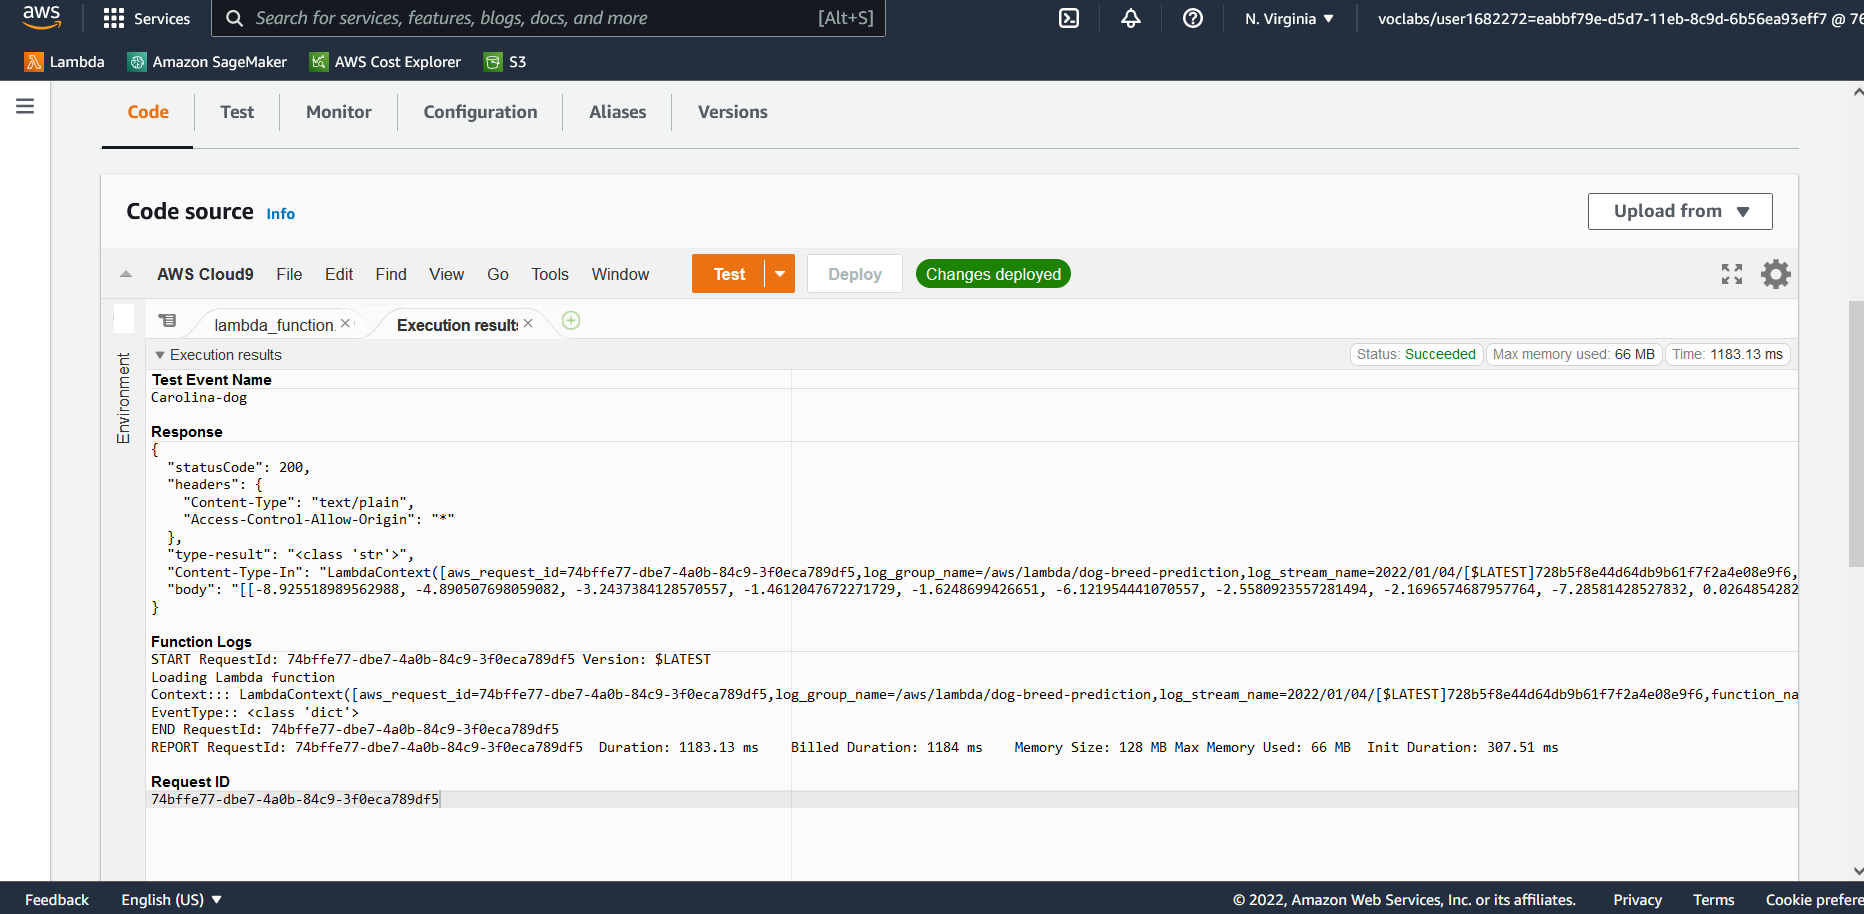
\includegraphics[width=\textwidth]{test_success.png}
\caption{Successful Lambda Test}
\label{fig:test}
\end{figure}
The highest number is in index 13, which means the model thinks this is most likely a Basenji. That's a decent guess, in my opinion, based on the body shape and coat type of the dog. The full test response can be found in the file \verb^lambda_test_results.txt^.
\subsection{Security}
I took a screenshot of the policies that are attached to my Lambda function's role (Fig \ref{fig:role}). In considering which policy to attach, I looked for one that would only allow the Lambda function to invoke endpoints, but I couldn't find one defined that narrowly. This is a vulnerability, since I've granted the Lambda function full access to SageMaker. This could be used to get or delete objects from S3, create or delete VPC endpoints in EC2, get metric data from CloudWatch, and list the secrets in Secrets Manager, among others. This suggests that we should be careful who is authorized to create Lambda functions in the first place, and we should regularly check the Access Advisor for roles to see which services are being accessed and when, to revoke the permissions if we see anything untoward. We should practice basic operational security around AWS accounts, such as multi-factor authentication, privileged account workstations, and regular active-user/role audits. I recognize all of the IAM roles and services accessed in my account, since it is nearly brand-new, but it's worth keeping an eye on.
\begin{figure}[h]
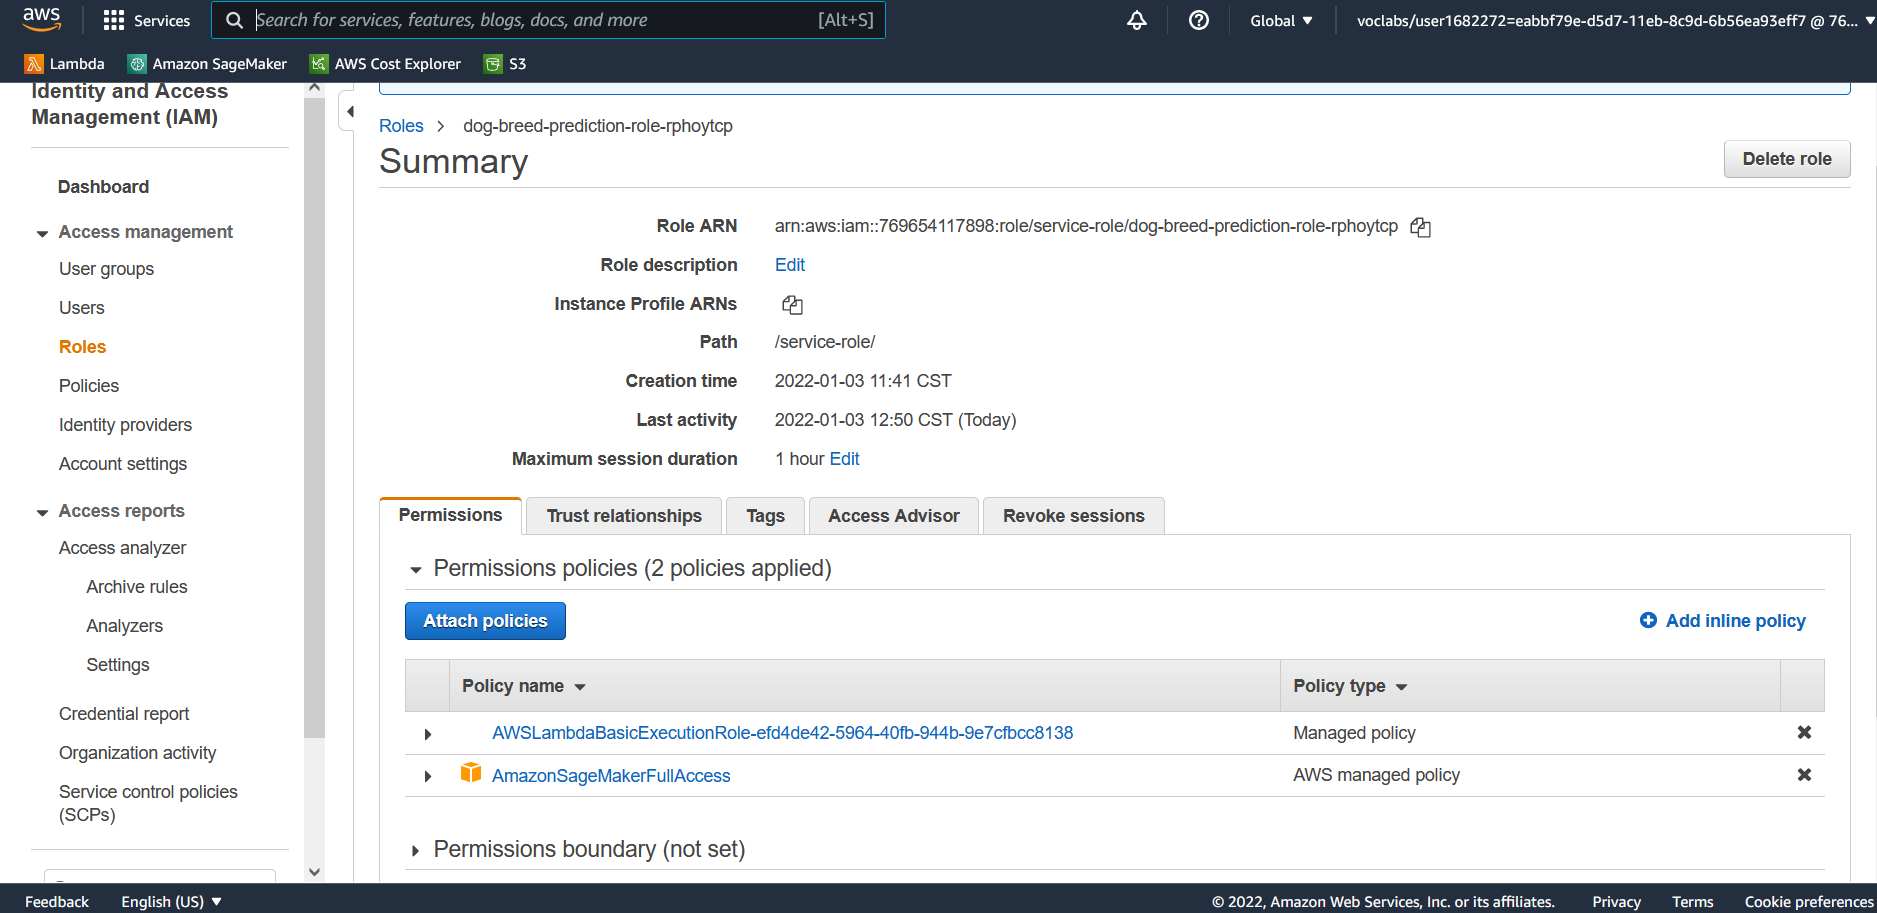
\includegraphics[width=\textwidth]{lambda_role.png}
\caption{Lambda Function IAM Role Policies}
\label{fig:role}
\end{figure}
\section{Concurrency and Auto-Scaling}
\subsection{Concurrency}
I configured a version of my Lambda function, and then I chose 3 reserved concurrency and 1 provisioned concurrency (Fig \ref{fig:concur}). I chose to add some of each kind of concurrency to demonstrate my knowledge, and these would be more than sufficient for my use of the Lambda function. Similarly, I configured auto-scaling for my deployed endpoint, with a min instance count of 1, a max of 3, and scale-in and scale-out cool down times of 30 seconds. Those settings were sufficient for the exercise we did earlier in the course, so I feel they're fine here as well.
\begin{figure}[h]
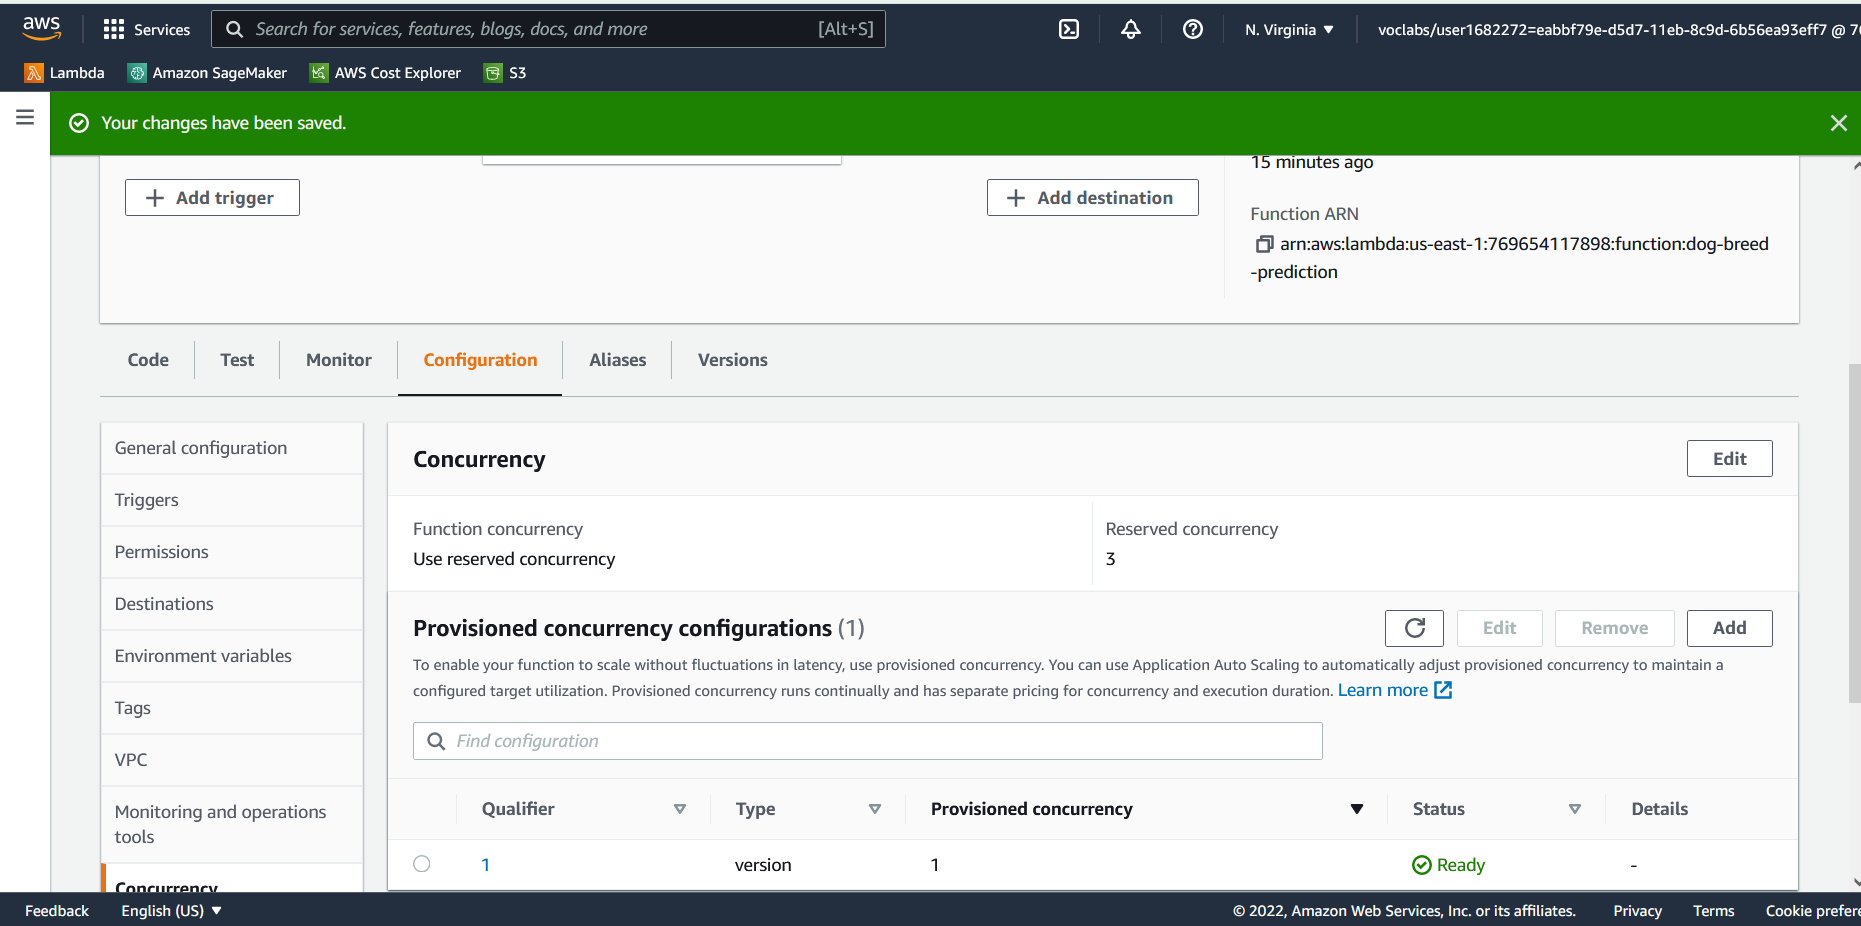
\includegraphics[width=\textwidth]{concurrency.png}
\caption{Lambda Concurrency Configuration}
\label{fig:concur}
\end{figure}

\vspace*{1in}
{\Large Thank you for your time!}
\end{document}

